\documentclass[12pt,aip,cha,reprint,nofootinbib]{revtex4-1}
\usepackage{amsfonts,amssymb,amsmath,times}%
\usepackage{graphicx}
\usepackage{bm}
\usepackage{enumerate}
\usepackage{color}

% \linespread{1}

\begin{document}

\title{Characterizing dynamical transitions by statistical complexity measures based on ordinal pattern transition networks} 

\author{Min Huang}
	\affiliation{School of Physics and Electronic Science, East China Normal University, Shanghai 200062, China}

\author{Zhongkui Sun}
	\affiliation{Department of Applied Mathematics, Northwestern Polytechnical University, Xi'an 710072, China}

\author{Jie Zhang}
	\affiliation{Institute of Science and Technology for Brain-Inspired Intellegence, Fudan University, Shanghai 200433,  China}

\author{Reik V. Donner}
        \affiliation{Department of Water, Environment, Construction and Safety, Magdeburg--Stendal University of Applied Sciences, Breitscheidstra{\ss}e 2, 39114 Magdeburg, Germany}
        \affiliation{Potsdam Institute for Climate Impact Research (PIK) -- Member of the Leibniz Society, Telegrafenberg A31, 14473 Potsdam, Germany}

\author{Shuguang Guan}
	\email[corresponding author: ]{sgguan@phy.ecnu.edu.cn}
	\affiliation{School of Physics and Electronic Science, East China Normal University, Shanghai 200062, China}
	
\author{Yong Zou}
	\email[corresponding author: ]{yzou@phy.ecnu.edu.cn}
	\affiliation{School of Physics and Electronic Science, East China Normal University, Shanghai 200062, China}

\date{\today}

\begin{abstract}
In the recent decade, complex network approaches are emerging as complementary novel ways to perform nonlinear time series analysis, in particular showing many insights that are hidden in the traditional methods. In this work, we focus on one of particular method of characterizing ordinal pattern transition network for time series data. More specifically, we generalize some traditional estimators of statistical complexity measures (SCM), which explicitly disclosing inhomogeneous frequencies of ordinal pattern transitions in the time series networks. To show the usefulness of the estimators, we use SCM to characterize different dynamical transitions, as illustrated by examples from the numerical model of  Logistic map and real time series of fluid experiments and ECG data. Both results of numerical and experimental data demonstrate that the transition frequencies between different ordinal patterns improve the SCM estimations, which are especially important for finite length of time series analysis, hence providing substantial information to the existing complex network approaches for nonlinear time series analysis. 
\end{abstract}

\pacs{05.45.Ac, 05.45.Tp, 89.75.Fb}
\maketitle

\section{Introduction}
In the recent decade, complex network based approaches have emerged as prominent tools for nonlinear time series analysis \cite{Kantz97,Sprott2003}, which have found many interesting applications to experimental data \cite{ZouPR2018}. For instance, 

There are several major methods are of particular importance, including recurrence network \cite{MarwanPLA2009,Donner2010a}, visibility graphs \cite{Lacasa2008,Nunez2012}, and transition networks \cite{Nicolis2005} and cycle network \cite{ZhangPRL2006}. Depending on the particular questions at hand, we note that each of these complex network approaches has various variants for different applications, for instance, constructing a single network for a univariate time series or interacting networks (multiplex or multilayer) networks for coupled time series. This line of research is undergoing fast developments for the time being as reviewed in \cite{ZouPR2018}. 

The focus of this paper is ordinal pattern transition networks. The advantages and some recent results. 

The basic idea of ordinal partition network method originates from identifying ordinal patterns of time series \cite{BandtPRL2002}, which is a well developed concept in nonlinear time series analysis. For instance, permutation entropy and the associated statistical analysis \cite{BandtPRL2002}. In addition, ordinal symbolic representation of time series has found a number of interesting applications in science and engineering, for instance, biomedical recordings \cite{AmigoPTRSA2014}, finance \cite{ZaninChaos2008}, climate sciences \cite{BarreiroChaos2011}. Some recent progress has been comprehensively reviewed in Ref. \cite{AmigoPTRSA2014}. More specifically, given a one-dimensional time series $\{ x(i)\}_{i=1, \cdots, L}$ comprising of $L$ sampled points from a dynamical system, we first reconstruct the corresponding phase space by time delay embedding $\vec{x}(i) = [x(i), x(i+\tau), \cdots, x(i+(D-1)\tau)]$ with dimension $D$ \cite{Takens1981,Kantz97}. Next, we represent each embedded phase point $\vec{x}(i)$ by its corresponding rank order, which is represented by a symbol $\pi_{i}$. When sliding windows from $i=1$ to $N = L - (D - 1)\tau$ in the embedded space, a symbolic representation of the trajectory $\pi_i$ is produced. It is possible to derive information about the dynamics of the underlying system by assessing different probabilities of ordinal patterns which is typical for a time series resulted from a deterministic system. More generally, we obtain a probability distribution $P$ whose elements $p(\pi_{i})$ are the frequencies associated to pattern $\pi_{i}$, $i = 1, \cdots, D!$. Clearly, $P$ provides a significant feasible way to estimate the probability distribution function for a given time series, which plays a crucial role in extracting statistical complexities of the underlying dynamical systems \cite{BandtPRL2002,AmigoPTRSA2014}. 

Relatively easy computation of $P$ by ordinal patterns for the underlying system prompts another successful application to compute statistical complexity measure \cite{kowalskiEntropy2011}. Traditionally, statistical complexity measures (SCMs) are defined as the product of the normalized Shannon entropy and disequilibrium \cite{kowalskiEntropy2011}, which capture specific organizational properties of structure and patterns in a process. Following the literature \cite{rossoPRL2007,LopezPLA1995,kowalskiEntropy2011}, in this work we consider Jensen-Shannon SCM which is defined as $\mathcal{C}_{JS}[P] = \mathcal{H}[P]  \cdot  Q_{JS}[P, P_e]$, where $\mathcal{H}[P]$ is the normalized Shannon entropy and $Q_{JS}[P, P_e]$ is the so-called disequilibrium function measuring the distance of the given $P$ to the uniform distribution $P_e$, i.e., by the Jensen-Shannon divergence. Thus, $Q_{JS}[P, P_e]$ is defined as $Q_{JS}[P, P_e] = Q_{0} \cdot JS[P, P_e]$ where $JS[P, P_e]$ is the Jensen-Shannon divergence between $P$ and $P_e$ and $Q_{0}$ is the normalization factor. Furthermore, the complexity-entropy plane $\mathcal{H} \times \mathcal{C}_{JS}$ has been intensively used to distinguish chaotic systems from stochastic ones \cite{rossoPRL2007}. The computation of the complexity-entropy planes has benefit from the ordinal pattern symbolization of time series and has found various applications \cite{rossoPRL2007,kowalskiEntropy2011}. However, in the complexity-entropy analysis, there are some chaotic maps that could be easily confused as random noise because no clear separable regions are available to differentiate dynamics as reported in \cite{BorgesAMC2019}. So far, it remains to be a challenging task to disclose the possible non-monotonic relationship between complexity and entropy \cite{MartinPLA2003}. 

Note that, in all above discussions of ordinal pattern analysis, the transition behavior between patterns remains largely unclear. Recently, ordinal partition network representations have been proposed to capture the transition behavior of the ordinal patterns \cite{MichaelChaos2015,KulpChaos2016,zhangSciRep2017,McCullough2017b,BorgesAMC2019}, which sheds novel insight on the standard ordinal symbolic analysis of time series. In particular, each ordinal pattern is considered as a vertex in the graph and a directed weighted edge connecting two patterns in the graph is established depending on the transition frequency. One of advantages of ordinal pattern transition networks is that we can provide pronounced distinction among different time series with short time series \cite{MichaelChaos2015,BorgesAMC2019}. 

In this work, we generalize the traditional statistical complexity measures by incorporating pattern transition probabilities. The advantages are the following: (i) All SCMs successfully show distinctions between different dynamics, including time series from numerical models and experimental data; (ii) These generalized SCMs help to capture the consistent relationship between statistical complexity measures and chaoticity; (iii) All SCMs are sensitive to dynamical transitions of period doubling, band merging, inner and outer crisis. 

The structure of the paper is organized as follows: In section \ref{sec:OPW}, we show two slightly different ways to obtain the transition matrix of the corresponding ordinal pattern transition networks. Furthermore, based on this matrix, we propose in section \ref{sec:SCM} to compute the statistical complexity measures from three different perspectives including static pattern frequency properties, dynamic pattern transition properties and both. We will use one example to emphasize the important effects of embedding parameters in section \ref{sec:embeddings}. The usefulness of SCMs will be illustrated by four time series of typical dynamical regimes of the Logistic map. In section \ref{sec:plane}, the traditional complexity-entropy planes of each SCM will be discussed while the control parameter is systematically changed. In order to characterize the dynamical transitions, we expand the SCM values versus the control parameter in section \ref{sec:transi}. Finally, we show that SCMs successfully distinguish different dynamical regimes by experimental time series from flow data and human ECG data in \ref{sec:time}. Some discussions will be provided in the last section \ref{sec:con}.  

\section{Ordinal pattern transition matrix} \label{sec:OPW}
Most of the current studies compute permutation entropy $\mathcal{S}_O$ focusing on the frequencies of ordinal patterns, which however overlooked the transition behavior between  patterns. To emphasize the transitions between any pair of two patterns, measures of transitional complexity have been further proposed in \cite{zhangSciRep2017,McCullough2017b} to quantify the resulting OPTNs. To this end, we indicate each directed link by its transition frequency $w_{ij} = p({\pi_i \to \pi_j})$, following the time iterations of the series. Calculating the transition frequency for each pattern, we obtain a weighted directed network characterized by a weighted adjacency matrix $W = \{ w_{ij} \}, i, j \in [1, D!]$. 

Based on the transition matrix $\mathbf{W}$ of an OPTN, we note that there two slightly different ways to introduce normalization factors in $W$. The first option is to use a global normalization to ensure $\sum_{i,j}^{D!} w_{ij} = 1$ \cite{zhangSciRep2017}, which results in a globally normalized transition entropy as termed below.  

The second option of normalization has been proposed by McCullough {\textit{et al}} \cite{McCullough2017b} that they first considered the local out-link transition frequency from pattern $\pi_i$ to $\pi_j$
\begin{equation} \label{eq:localTp}
p_{\pi_i \to \pi_j} = \left \{ \begin{aligned}
				& 0,  \;\;\;\;\;\;\;\;\;\;\;\;\;\;\;\;\;\;\;\;\; \text{if} \;\;\; \pi_i = \pi_j \\
				& \frac{w_{ij}}{\sum_{j, j \neq i} w_{ij}}, \;\;\;\;\;\; \text{if} \; \pi_i \neq \pi_j.\\
				\end{aligned}
				\right.
\end{equation}		
Note that the transition frequency of Eq.~\eqref{eq:localTp} is pattern (row-) wise normalized. This case will be referred to as node-wise out-link normalized transition matrix $\mathbf{W}$ in the following. In this way, it easily captures heterogeneous behavior of both static frequencies of different patterns and dynamic transition frequencies between patterns. 

In addition, we need to consider self-loops that may affect the numerical estimation of $\mathbf{W}$ which is especially important for time series from continuous systems. More specifically, it has been demonstrated in \cite{zhangSciRep2017} that there are about $99\%$ self-loops in the time series of R\"ossler system integrated by a step size $h = 0.01$, while about $1\%$ non-self-loops are hidden in $\mathbf{W}$. In addition, self-loops are related to the temporal correlation of time series \cite{BorgesAMC2019}. On the other hand, neglecting self-loops in $\mathbf{W}$ emphasizes the transition behavior between different patterns, which follows most of the existing studies of complex networks for computational simplicity and theoretical concerns \cite{CostaADPhy2007}. Therefore, we remove self-loops before computing the weighted matrix $\mathbf{W}$. In other cases of stochastic processes and discrete systems, self-loops have been included in the analysis showing some interesting results $\mathbf{W}$ \cite{BorgesAMC2019}. We argue that whether to remove or to consider self-loops depends on the particular processes under study. Anyway, we have verified that our results below do not change significantly while considering effects of self-loops.

\section{Statistical complexity measures} \label{sec:SCM}
In this section, we review briefly ordinal pattern frequency based SCM and propose two novel ways to define SCM, which explicitly consider transition frequencies of the resulting ordinal network representations for time series. 
 
$\bullet$ SCM based on permutation entropy of pattern frequencies. 

The permutation entropy of a time series is the Shannon entropy of the distribution of patterns $P = \{p_{\pi_1}, p_{\pi_2}, \cdots, p_{\pi_i} \}$, which is computed as
\begin{equation}
\mathcal{S}_{O}[P]= - \sum_{i=1}^{D!} p_{\pi_i} \log p_{\pi_i}. 
\end{equation}
The normalized permutation entropy $\mathcal{H}_O$ is defined as 
\begin{equation} \label{eq:Ho}
\mathcal{H}_{O}[P] = \mathcal{S}_{O}[P] / \mathcal{S}_{O, max}, 
\end{equation}
where $\mathcal{S}_{O, max} = \log D!$ is resulted from the case of uniform distribution of the same number of patterns $P_e = \{1/D!, \cdots, 1/D!\}$.  In the next step, we use some distance definition to measure the given $P$ to the uniform distribution $P_e$, which is the core of statistical complexity measures (SCM).  There are several different distance functions as illustrated in the literature, such as Euclidean norm, Wooters' distance, Kullback-Leibler relative entropy and Jensen-Shannon divergence \cite{kowalskiEntropy2011}. In this work, the difference between the distribution $P$ and $P_e$ is characterized by the Jensen-Shannon divergence $Q_{JS}[P] = Q_0 \cdot JS[P, P_e]$ where $JS[P, P_e]$ is calculated by 
\begin{equation}
JS[P, P_e] = \mathcal{S}_O[\frac{P+P_e}{2}] - \frac{1}{2}\mathcal{S}_O[P] - \frac{1}{2}\mathcal{S}_O[P_e], 
\end{equation}
where $Q_0$ is a normalization factor with its value equal to the inverse of the maximal distance $JS[P, P_e]$, which ensures $Q_{JS}[P] \in [0, 1]$. This maximal distance is obtained when the distribution $P$ has probability one at one pattern and zeros at all other patterns. The general expression of $Q_0$ reads  
\begin{equation} \label{eq:Q0}
Q_0 = -2 \{(\frac{N+1}{N}) \log (N+1) -2 \log (2N) + \log (N)  \}^{-1}
\end{equation}
where $N = D!$ is the number of maximal patterns. For large $D$, we have $Q_0 \approx 1 /  \log 2$. 

The function $Q_{JS}[P]$ is different from zero if the system has a kind of privilege over patterns among the accessible ones, reflecting determinism of the system. Finally, the SCM based on permutation entropy of node (pattern) frequencies is defined as 
\begin{equation}
\mathcal{C}_{O}[P] = Q_{JS}[P] \cdot \mathcal{H}_{O}[P].
\end{equation}
This quantity is static in the sense that it quantifies the amount of information stored by ordinal frequencies in the system and its disequilibrium of the observed parts of its accessible states in comparison to uniform distribution \cite{LopezPLA1995}. 

$\bullet$ SCM based on transition entropy by globally normalized weighting matrix $W$. 

In this case, the sum of all entries of the transition matrix $W$ is 1 and the Shannon entropy of transition frequencies between any pair of ordinal patterns is therefore 
\begin{equation}
\begin{split}
\mathcal{S}_{W}[W] &= - \sum_{i=1}^{D!} \sum_{j = 1; j \neq i}^{D!} w_{ij} \log w_{ij}, \\
& = - \sum_{i=1}^{D!} \sum_{j =1; j \neq i}^{D!} p_{\pi_i \to \pi_j} \log p_{\pi_i \to \pi_j}. 
\end{split}
\end{equation}
The normalized entropy is hence defined 
\begin{equation}
\mathcal{H}_{W}[W] = \mathcal{S}_{W}[W] / \mathcal{S}_{W, max}, 
\end{equation}
where $\mathcal{S}_{W, max} = \log D! (D! - 1)$ and the self transitions are excluded. Furthermore, there are $D! (D! - 1)$ pattern transitions in the uniformly distribution function $P_e$. Thus, in a full analogy with node-based SCM, the Jensen-Shannon distance is therefore computed as $Q_{JS}[W] = Q_0 \cdot JS[W, P_e]$, where $JS[W, P_e]$ is computed as 
\begin{equation}
JS [W, P_e] = \mathcal{S}_{W}[\frac{W + P_e}{2}] - \frac{1}{2}\mathcal{S}_{W}[W] - \frac{1}{2}\mathcal{S}_{W}[P_e]. 
\end{equation}
We note that we have the same expression of the normalization factor $Q_0$ while replacing $N = D! (D! - 1)$ in Eq. \eqref{eq:Q0}. This further yields the SCM 
\begin{equation}
\mathcal{C}_{W}[W] = Q_{JS}[W] \cdot \mathcal{H}_{W}[W].
\end{equation}
This quantify is dynamic in the sense that it considers the state transition information stored in the system. 


$\bullet$ SCM based on transition entropy by node-wise out-edge normalized
weighting matrix $W$.

In this case, the ordinal transition matrix is node-wised normalized, i.e., row
sum of $W$ is 1. Therefore, we first introduce node-wise out-edge transition entropy which is calculated 
\begin{equation}
\begin{split}
\mathcal{S}_{E}^{\pi_i}[W_{\pi_i}] &= - \sum_{j = 1; j \neq i}^{D!} w_{ij} \log w_{ij},  \\ 
&= - \sum_{j=1, j \neq i}^{D!} p_{\pi_i \to \pi_j} \log p_{\pi_i \to \pi_j}. 
\end{split}
\end{equation}
Furthermore, node-wise normalized transition entropy is 
\begin{equation}
\mathcal{H}_{E}^{\pi_i}[W_{\pi_i}] = \mathcal{S}_{E}^{\pi_i}[W_{\pi_i}] / \mathcal{S}_{E, max}, 
\end{equation}
where $\mathcal{S}_{E, max} = \log (D! - 1)$. Note that this normalization factor is the same for all patterns, namely, $\mathcal{S}_{E, max}^{\pi_i} = \mathcal{S}_{E, max}^{\pi_j}$ and, therefore, the superscript is suppressed in the above definition. In addition, node-wise Jensen-Shannon distance is defined as $Q_{JS}^{\pi_i}[W_{\pi_i}] = Q_0 \cdot JS^{\pi_i} [W_{\pi_i}, P_e]$, where the disequilibrium 
\begin{equation}
JS^{\pi_i} [W_{\pi_i}, P_e] = \mathcal{S}_{E}^{\pi_i}[\frac{W_{\pi_i} + P_e}{2}] - \frac{1}{2}\mathcal{S}_{E}^{\pi_i}[W_{\pi_i}] - \frac{1}{2}\mathcal{S}_{E}^{\pi_i}[P_e]. 
\end{equation}
In this case, we note that we have the normalization factor $Q_0$ while replacing $N = D! - 1$ in Eq. \eqref{eq:Q0}. Taking into account node frequencies, the global Jensen-Shannon divergence is computed as 
\begin{equation}
Q_{JS}[W, P_e] = \sum_{i=1}^{D!} p(\pi_i) Q_{JS}^{\pi_i}[W_{\pi_i}], 
\end{equation}
which therefore yields an alternative definition of SCM of the transition network 
\begin{equation}
\mathcal{C}_{E}[W] = Q_{JS}[W, P_e] \cdot \mathcal{H}_{E}[W], 
\end{equation}
where $\mathcal{H}_{E}[W] = \sum_{i} p(\pi_i) \mathcal{H}_{E}^{\pi_i}[W_{\pi_i}]$. This quantity is dynamic in the sense that it quantifies both the static ordinal state frequencies and the dynamic state transition information stored in the system. 

\section{Choice of embedding parameters} \label{sec:embeddings}
There are two important algorithmic parameters in constructing ordinal pattern transition networks, namely, embedding parameters of $D$ and $\tau$. In some cases, the choice of $D$ and $\tau$ may strongly change the results since $D$ and $\tau$ should compromise the time scales of the respective time series. In general applications of ordinal pattern analysis (i.e., permutation entropy computation $\mathcal{S}_O$), the choice of optimal $D$ and $\tau$ depends on the field of application, which requires experience of experts as systematically summarized in \cite{Riedl2013}.
\begin{figure*}
	\centering 
	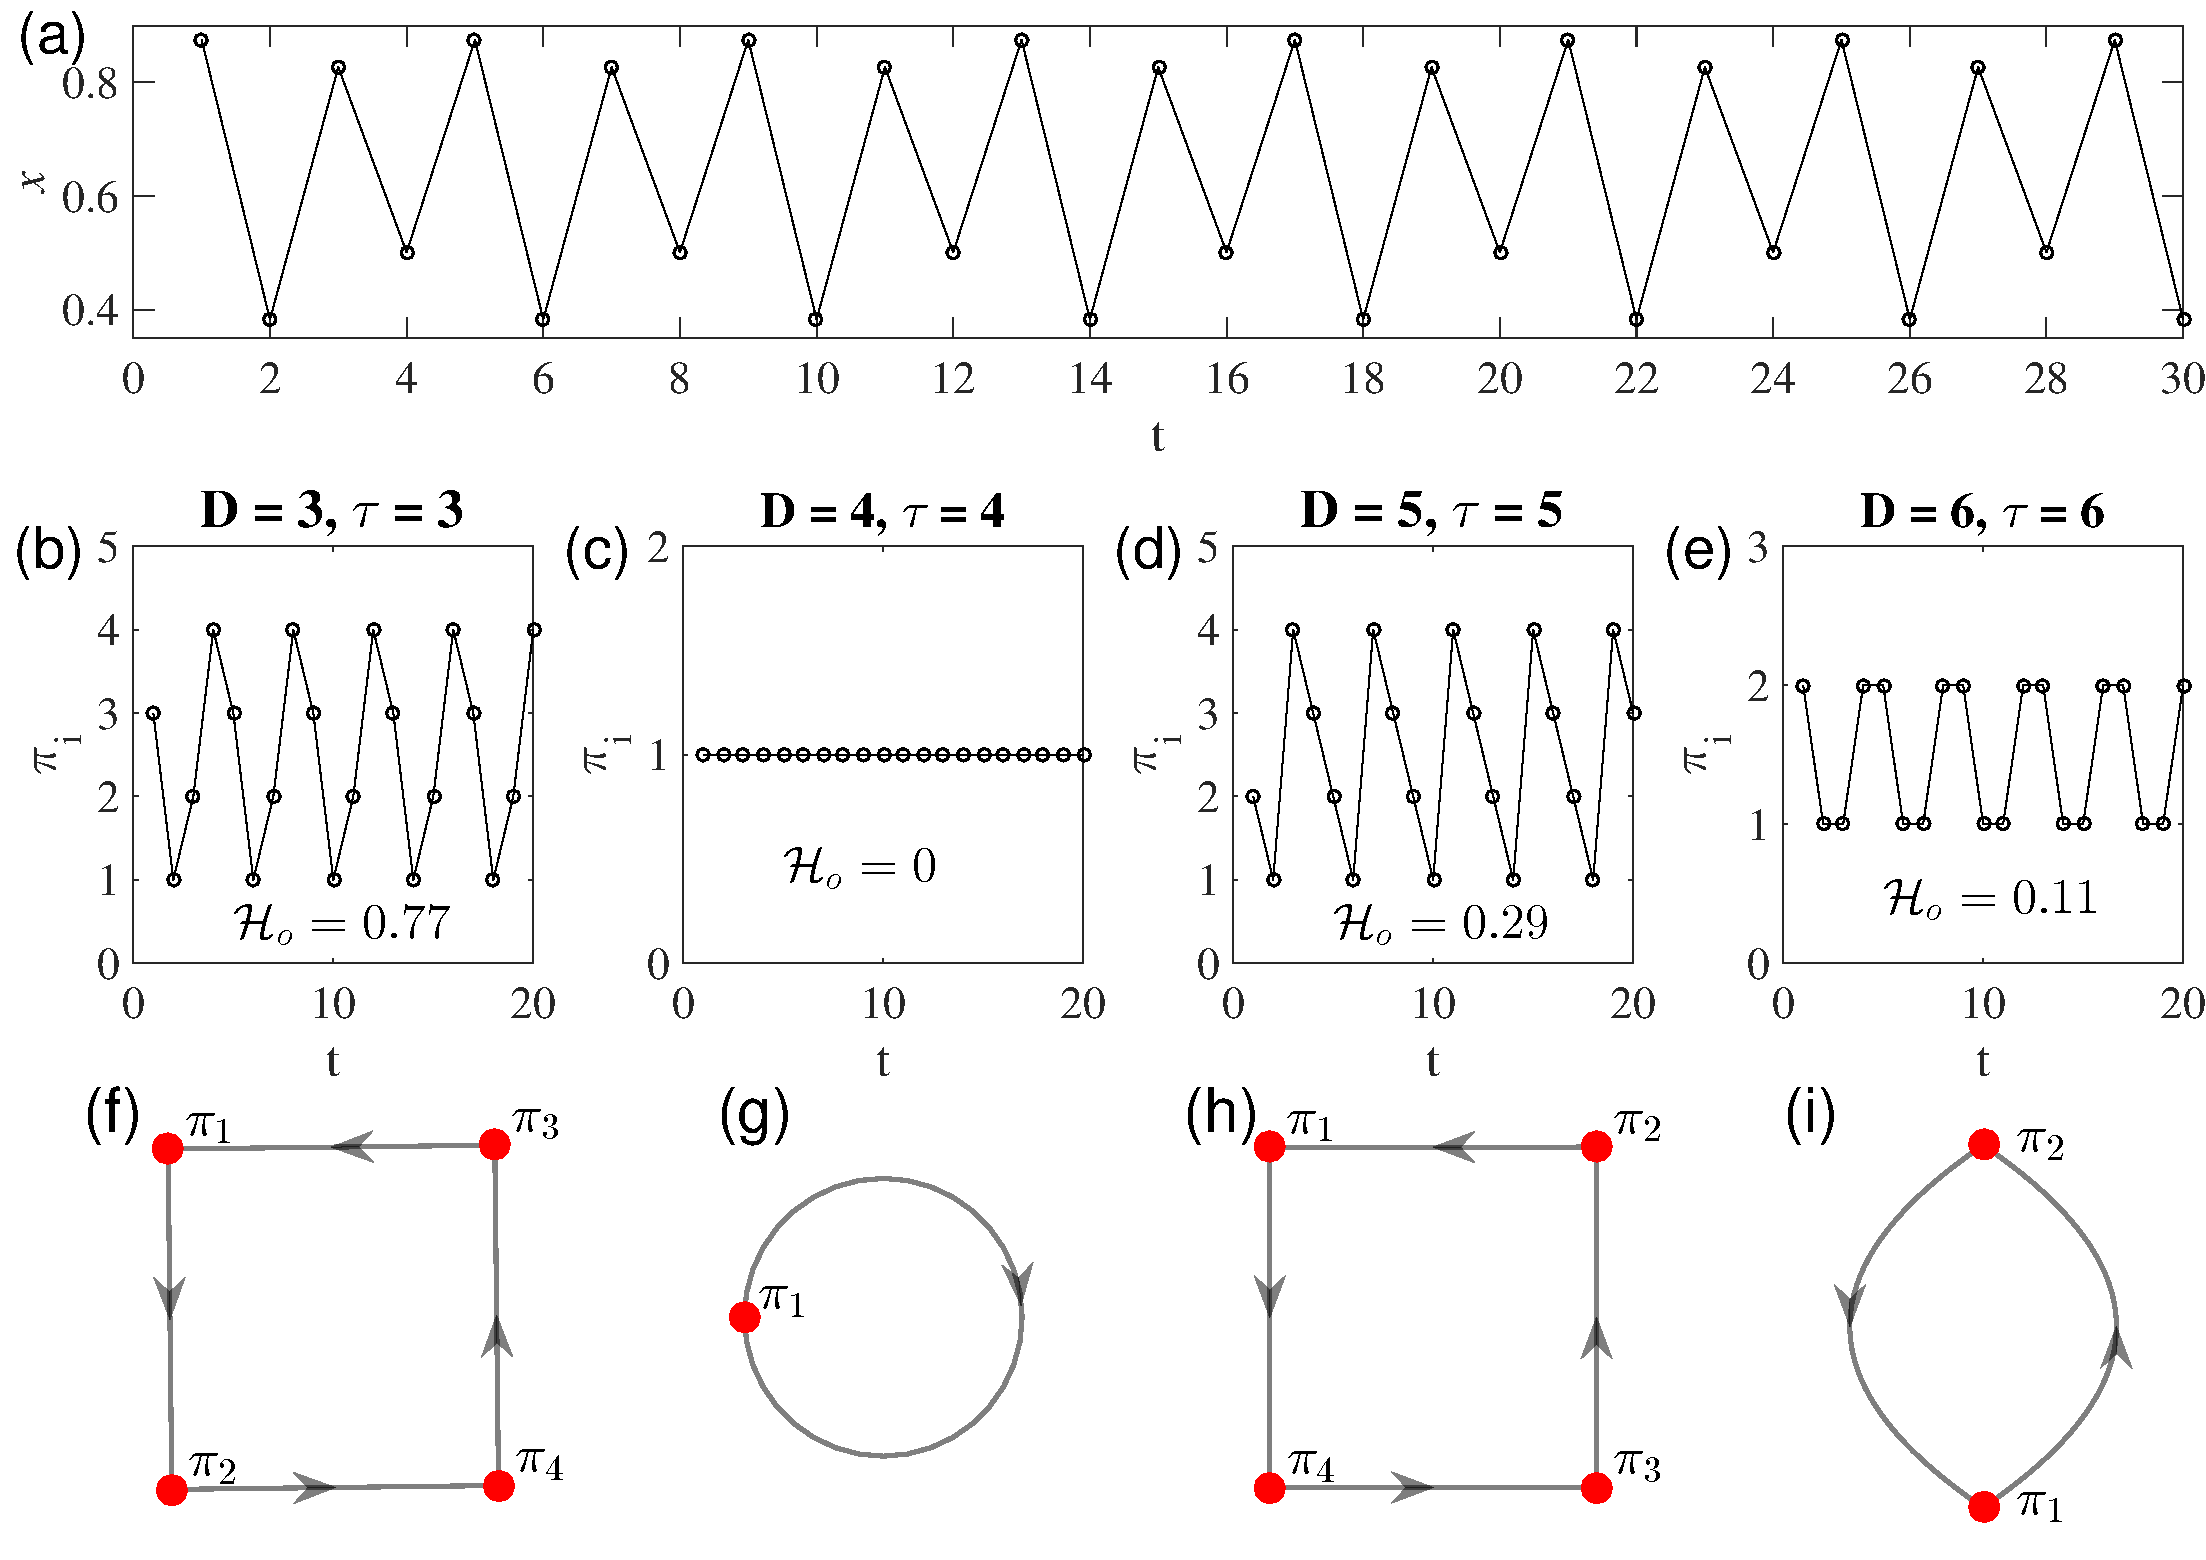
\includegraphics[width=2\columnwidth]{period4_logisticExample.pdf}
\caption{\small{Example of a period-4 iterative time series ($r= 3.5$ in the Logistic map) to show the effects of embedding parameters $D$ and $\tau$. (a) iterative time series and the corresponding ordinal pattern series by different $D$ and $\tau$, (b) $D = \tau = 3$, (c) $D = \tau = 4$, (d) $D = \tau = 5$, and (e) $D = \tau = 6$. The respective permutation entropy values normalized by $\log D!$ as Eq. \eqref{eq:Ho} are $\mathcal{H}_O = 0.77$, $0$, $0.29$, and $0.11$ as indicated in the insets of each panel. (f-i) show the corresponding ordinal pattern transition networks. The weights of directed edges are suppressed due to two slightly different normalizations are introduced. Note in (g), only self-loops are available since $D = \tau = 4$ result in a unique pattern. Missing patterns are suppressed. }
\label{fig:embed}}
\end{figure*}
Here we use one example to show the important roles of $D$ and $\tau$ for a period-4 time series in Figure \ref{fig:embed}. In this example, we choose $D = \tau $ and the corresponding ordinal pattern series are significantly influenced by these parameter settings, which further result in different permutation entropy values of $\mathcal{H}_O$.  For instance, only one unique ordinal pattern is observed when $D = \tau = 4$ (Fig. \ref{fig:embed}(c, g)) resulting in $\mathcal{H}_O = 0$, which is due to the coverage of one full period by the particular embedding parameters. Other values of $D$ and $\tau$ yield non-zero entropy values. The results of Fig. \ref{fig:embed} seem to be pessimistic since $D$ and $\tau$ will change the positions in the complexity-entropy planes. In the special case of the logistic map, we do not have a unique choice of $D$ and $\tau$ for periodic windows when the control parameter $r$ is varied. In such cases, we should focus more on the transitions between different dynamic regimes. Instead, we show that the results are robust when the control parameters are systematically changed while using the same parameter settings of $D$ and $\tau$.

\section{Results for four typical dynamic regimes} \label{sec:four}
We illustrate the potential of the proposed SCMs to characterize different dynamical regimes and transitions by analysis of the Logistic map $x_{n+1} = r x_n (1 - x_n)$ with the control parameter in the interesting range of $r \in [3.5, 4]$ with a step size of $\Delta r = 0.001$. In the range of the parameter $r$, various dynamical regimes and transitions between them can be found, for instance, period doublings, band merging points, inner and outer crises, intermittency \cite{Kantz97}, which has been served as a pragmatic model for nonlinear time series \cite{MarwanPLA2009}. 

First, we show several typical regimes of particular control parameter $r$, i.e., periodic dynamics, band merging, laminar states and outer crisis, we investigate the SCMs in more detail which have been summarized in Tab \ref{tableLog}. We note that several chaos-chaos transitions have been discussed in the following, namely, the band merging corresponds to intermittency, the inner crisis to certain chaos-chaos transition and the outer crisis to fully chaotic dynamics. 
\begin{table}[htb]
    {\begin{tabular}{l  l  l  l  l  l  l  l}
    \hline
    Regime & $r$      & $\mathcal{H}_O$ & $\mathcal{C}_O$ & $\mathcal{H}_W$ & $\mathcal{C}_W$ & $\mathcal{H}_E$   & $\mathcal{C}_E$  \\
    \hline
    Period 3      & 3.83 & 0 & 0 & 0 & 0 & 0 & 0 \\
    \hline
    Band merge    & 3.679 & 0.978 & 0.043 & 0.595 & 577 & 0.211 & 0.205  \\
    \hline
    Laminarity    & 3.791 & 0.986 & 0.029 & 0.633 & 0.609 & 0.280 & 0.269 \\
    \hline
    Outer crisis  & 4.0 & 0.994 & 0.014 & 0.677 & 0.638 & 0.359 & 0.339 \\
    \hline
    \end{tabular}}
   \caption{Statistical complexity measures for four different control parameters of the Logistic map (embedding parameters: $D = \tau = 6$).   \label{tableLog}}    
\end{table}
In Tab. \ref{tableLog}, we have used embeddings $D = \tau = 6$. Therefore, all SCMs values are zeros for period-3 series because each embedded vector covers two full periods (c.f., Fig. \ref{fig:embed}). Other choice of $D$ and $\tau$ often yields non-zero values for period-3 regime as discussed in Fig.\ref{fig:embed}. For other cases of band merging, laminarity and outer crisis, all SCMs values are significantly larger than zeros. The pattern frequency based SCMs of $\mathcal{C}_O$ show smaller values for all regimes, which further lead to the lower right locations in the complexity-entropy planes in Fig. \ref{fig:fBmNoise}(a). However, for transition matrix based SCMs, their entropy $\mathcal{H}_W$, $\mathcal{H}_E$ and complexity $\mathcal{C}_W$, $\mathcal{C}_E$ show more consistent results while considering the chaoticity level of the system. In particular, SCMs are the largest when $r = 4$ in the outer crisis regime, and the SCMs are the smallest when $r = 3.679$ in the band merging case, while the laminarity regime has the intermediate SCM values. 

\section{Results on complexity-entropy planes} \label{sec:plane}
In this section, we show the complexity-entropy planes by varying the control parameter $r$ in the illustrative Logistic model.  Note that the Logistic map has been discussed in the framework of SCM \cite{RossoPRE2007,MartinPLA2003}, but only for pattern frequency based complexity. For each control parameter $r$, we construct ordinal pattern transition network from a time series of length $L = 31000$. In order to exclude transient behavior we remove the first $1000$ values from the data series. We have repeated the following calculations for embeddings $D = \tau \in [2, 7]$. 

When only one unique ordinal pattern is identified following the time series, we set the SCMs values $0$, which is reasonable since only self-loop is observed. This happens only if $D$ is an integer factor of the period for periodic windows of the Logistic map (e.g., Fig. \ref{fig:embed}(g)).  Another notion is the data requirements for computing entropies and complexity measures. For reliable estimation of SCMs, a condition of the length of time series $L$ larger than $D!$ has been satisfied while $3 \leq D \leq 7$\cite{rossoPRL2007,kowalskiPhyD2007}. In the particular example of Logistic map, one may use longer data lengths (i.e., we have tested it up to $5 \times 10^6$), but this does not improve the estimate very much. 

Traditionally, SCM have been applied to distinguish chaos from noise by means of the complexity-entropy plane. In particular, this plane shows the statistical complexity measures ($\mathcal{C}_O$, $\mathcal{C}_W$ and $\mathcal{C}_E$) as a function of the corresponding normalized entropy values ($\mathcal{H}_O$, $\mathcal{H}_W$ and $\mathcal{H}_E$). The above SCMs quantify both randomness and correlation structures of time series, which in consequence result in a non-trivial function of entropy  values. Chaotic systems present maximal complexity while stochastic systems have lower values of complexity, hence presenting in different regions in the complexity-entropy plane\cite{rossoPRL2007}. Furthermore, SCM values lie in a range of a minimum $\mathcal{C}_{min}$ and a maximum $\mathcal{C}_{max}$. A general algorithm for computing the bounds $\mathcal{C}_{min}$ and $\mathcal{C}_{max}$ is provided in \cite{martinPhyA2006}. Figure \ref{fig:fBmNoise} shows the complexity-entropy planes for embedding parameters $D = \tau = 6$. We emphasize that the results in Fig. \ref{fig:fBmNoise} are qualitatively the same when $D$ and $\tau$ are varied in the interval $[3, 7]$, and we choose $D = 4, 5, 6$ as illustrative examples as shown in Fig. \ref{fig:fBmNoise}. Furthermore, the computation of $\mathcal{C}_{max}$ depends on the embedding $D$ since $D$ determines the number of patterns and pattern transitions which are included in the definition of SCMs. However, $\mathcal{C}_{min}$ shows less dependence on $D$. 
\begin{figure*}
	\centering 
	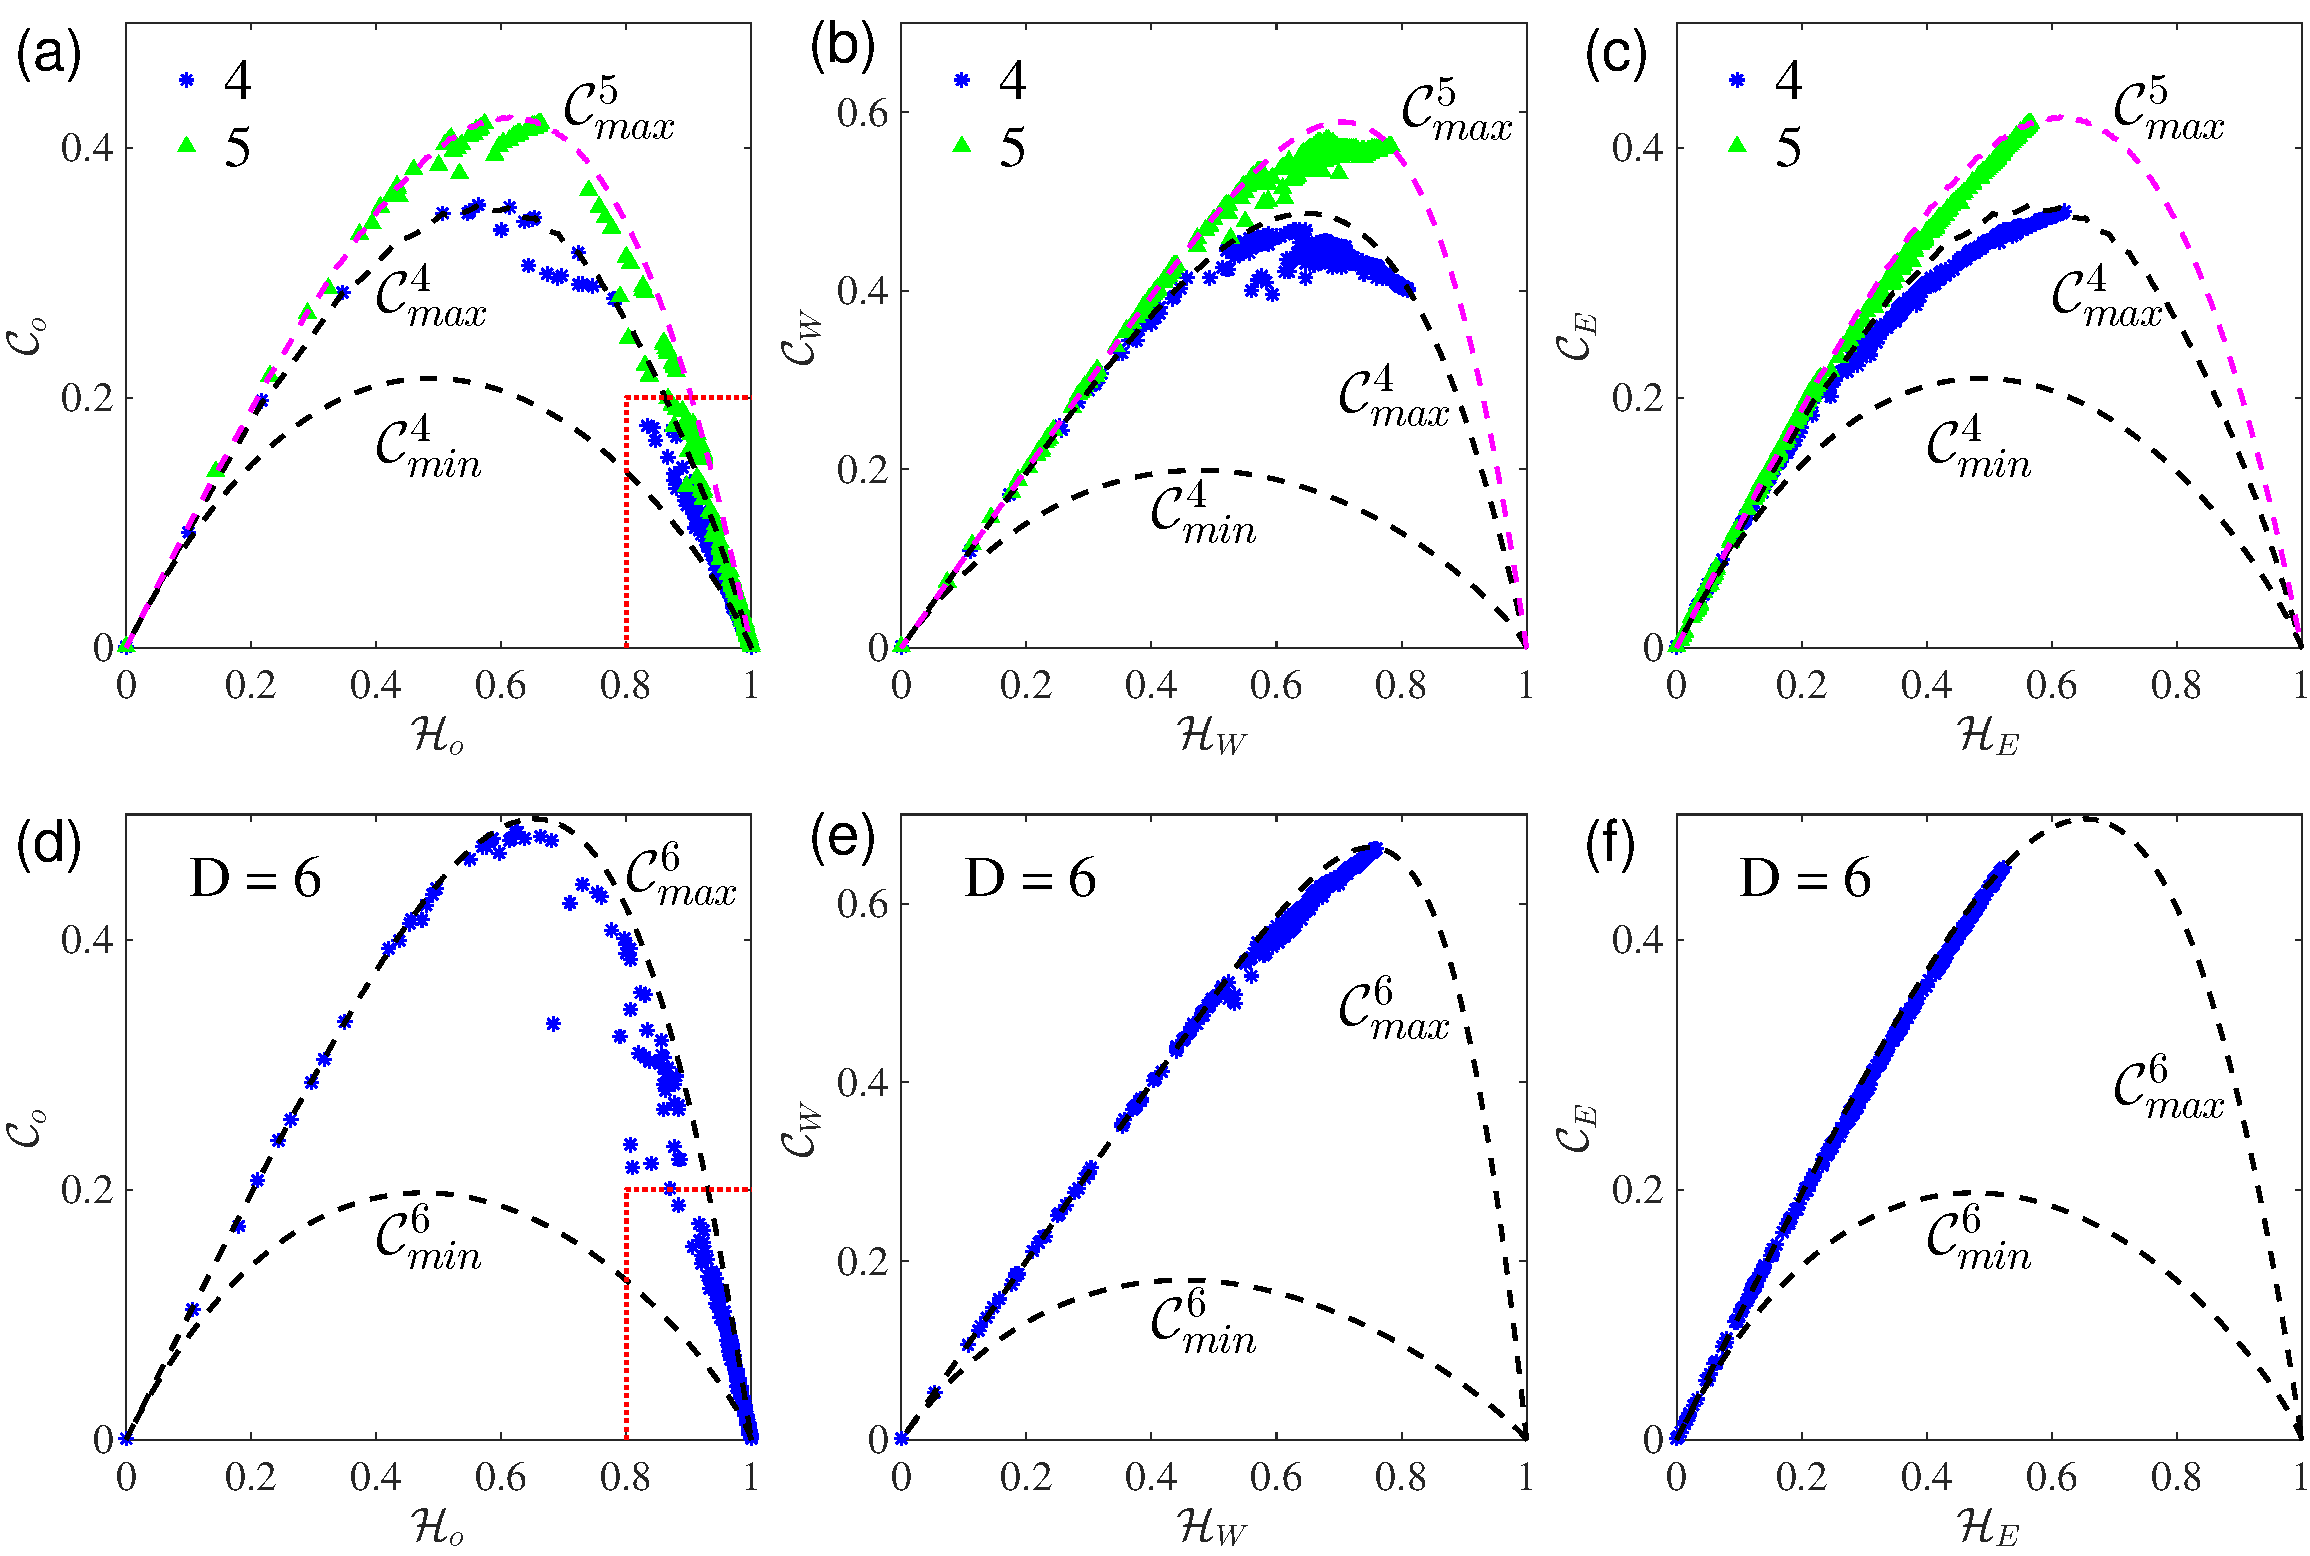
\includegraphics[width=2\columnwidth]{CompEntropy_LogisticHC.pdf}
\caption{\small{Complexity-entropy planes (Jensen-Shannon divergence) to show statistical complexity measures for example series of the logistic map for varying the control parameter $r$. (a, d) $\mathcal{C}_O$ versus $\mathcal{H}_O$, (b, e) $\mathcal{C}_{W}$ versus $\mathcal{H}_{W}$, and (c, f) $\mathcal{C}_{E}$ versus $\mathcal{H}_{E}$. The dashed lines correspond to the maximum $\mathcal{C}_{max}$ and minimum complexity $\mathcal{C}_{min}$ values for a fixed value of the entropy. (a-c) for embedding $D = 4, 5$ and (d-f) for $D = 6$. In (a, d), the bottom-right rectangles of dotted lines highlighted the ambiguous regions for the traditional pattern frequency based SCM analysis. }  \label{fig:fBmNoise}}
\end{figure*}

In this complexity-entropy plane, pattern frequency based SCM values lie around the maximum curve $\mathcal{C}_{max}$. It is clear to see that the displacements of the dots depend on the embedding $D$ as shown in Fig. \ref{fig:fBmNoise}(a, d). In addition, there are many dots in the bottom-right position of the plane, which have been highlighted by rectangles of dotted lines. Indeed, this is a challenging region for SCMs to distinguish chaotic time series from random noise in Fig. \ref{fig:fBmNoise}(a, d), which has been reported in \cite{BorgesAMC2019}, too. It is not an easy task to correctly tell the difference between chaos (i.e., chaotic regimes of large $r$ in the Logistic map) and noise. This is because the SCMs of $\mathcal{H}_O$ and $\mathcal{C}_O$ are static in the sense that only pattern frequencies have been considered in the definitions. The results that  $\mathcal{H}_O$ and $\mathcal{C}_O$ are displaced close to $\mathcal{C}_{max}$ curves have been observed when the embedding $D$ is increased (Fig. \ref{fig:fBmNoise}(a, d)). 

For other pattern transition based SCMs of $\mathcal{C}_W$ vs $\mathcal{H}_W$ and $\mathcal{C}_E$ vs $\mathcal{H}_E$, we also find that the dots are distributed close to the respective maximum lines of $\mathcal{C}_{max}$. Increasing the embedding dimension further to $D=6, 7$, the dots are covered by the left uprising branch the parabola curve $\mathcal{C}_{max}$ (Fig. \ref{fig:fBmNoise}(b, d)). The definition of $\mathcal{C}_{E}$ and $\mathcal{H}_{E}$ takes into account the information of both pattern frequencies and pattern transitions, which results in that the dots are closer to $\mathcal{C}_{max}$ in a relative faster manner (Fig. \ref{fig:fBmNoise}(c, f)). The most interesting result is that no points lie in the bottom-right challenging regions of ambiguity. It is the deterministic transition behavior among patterns that makes the distinction from random noise. 

%For a better comparison 
%\begin{figure*}
%	\centering 
%	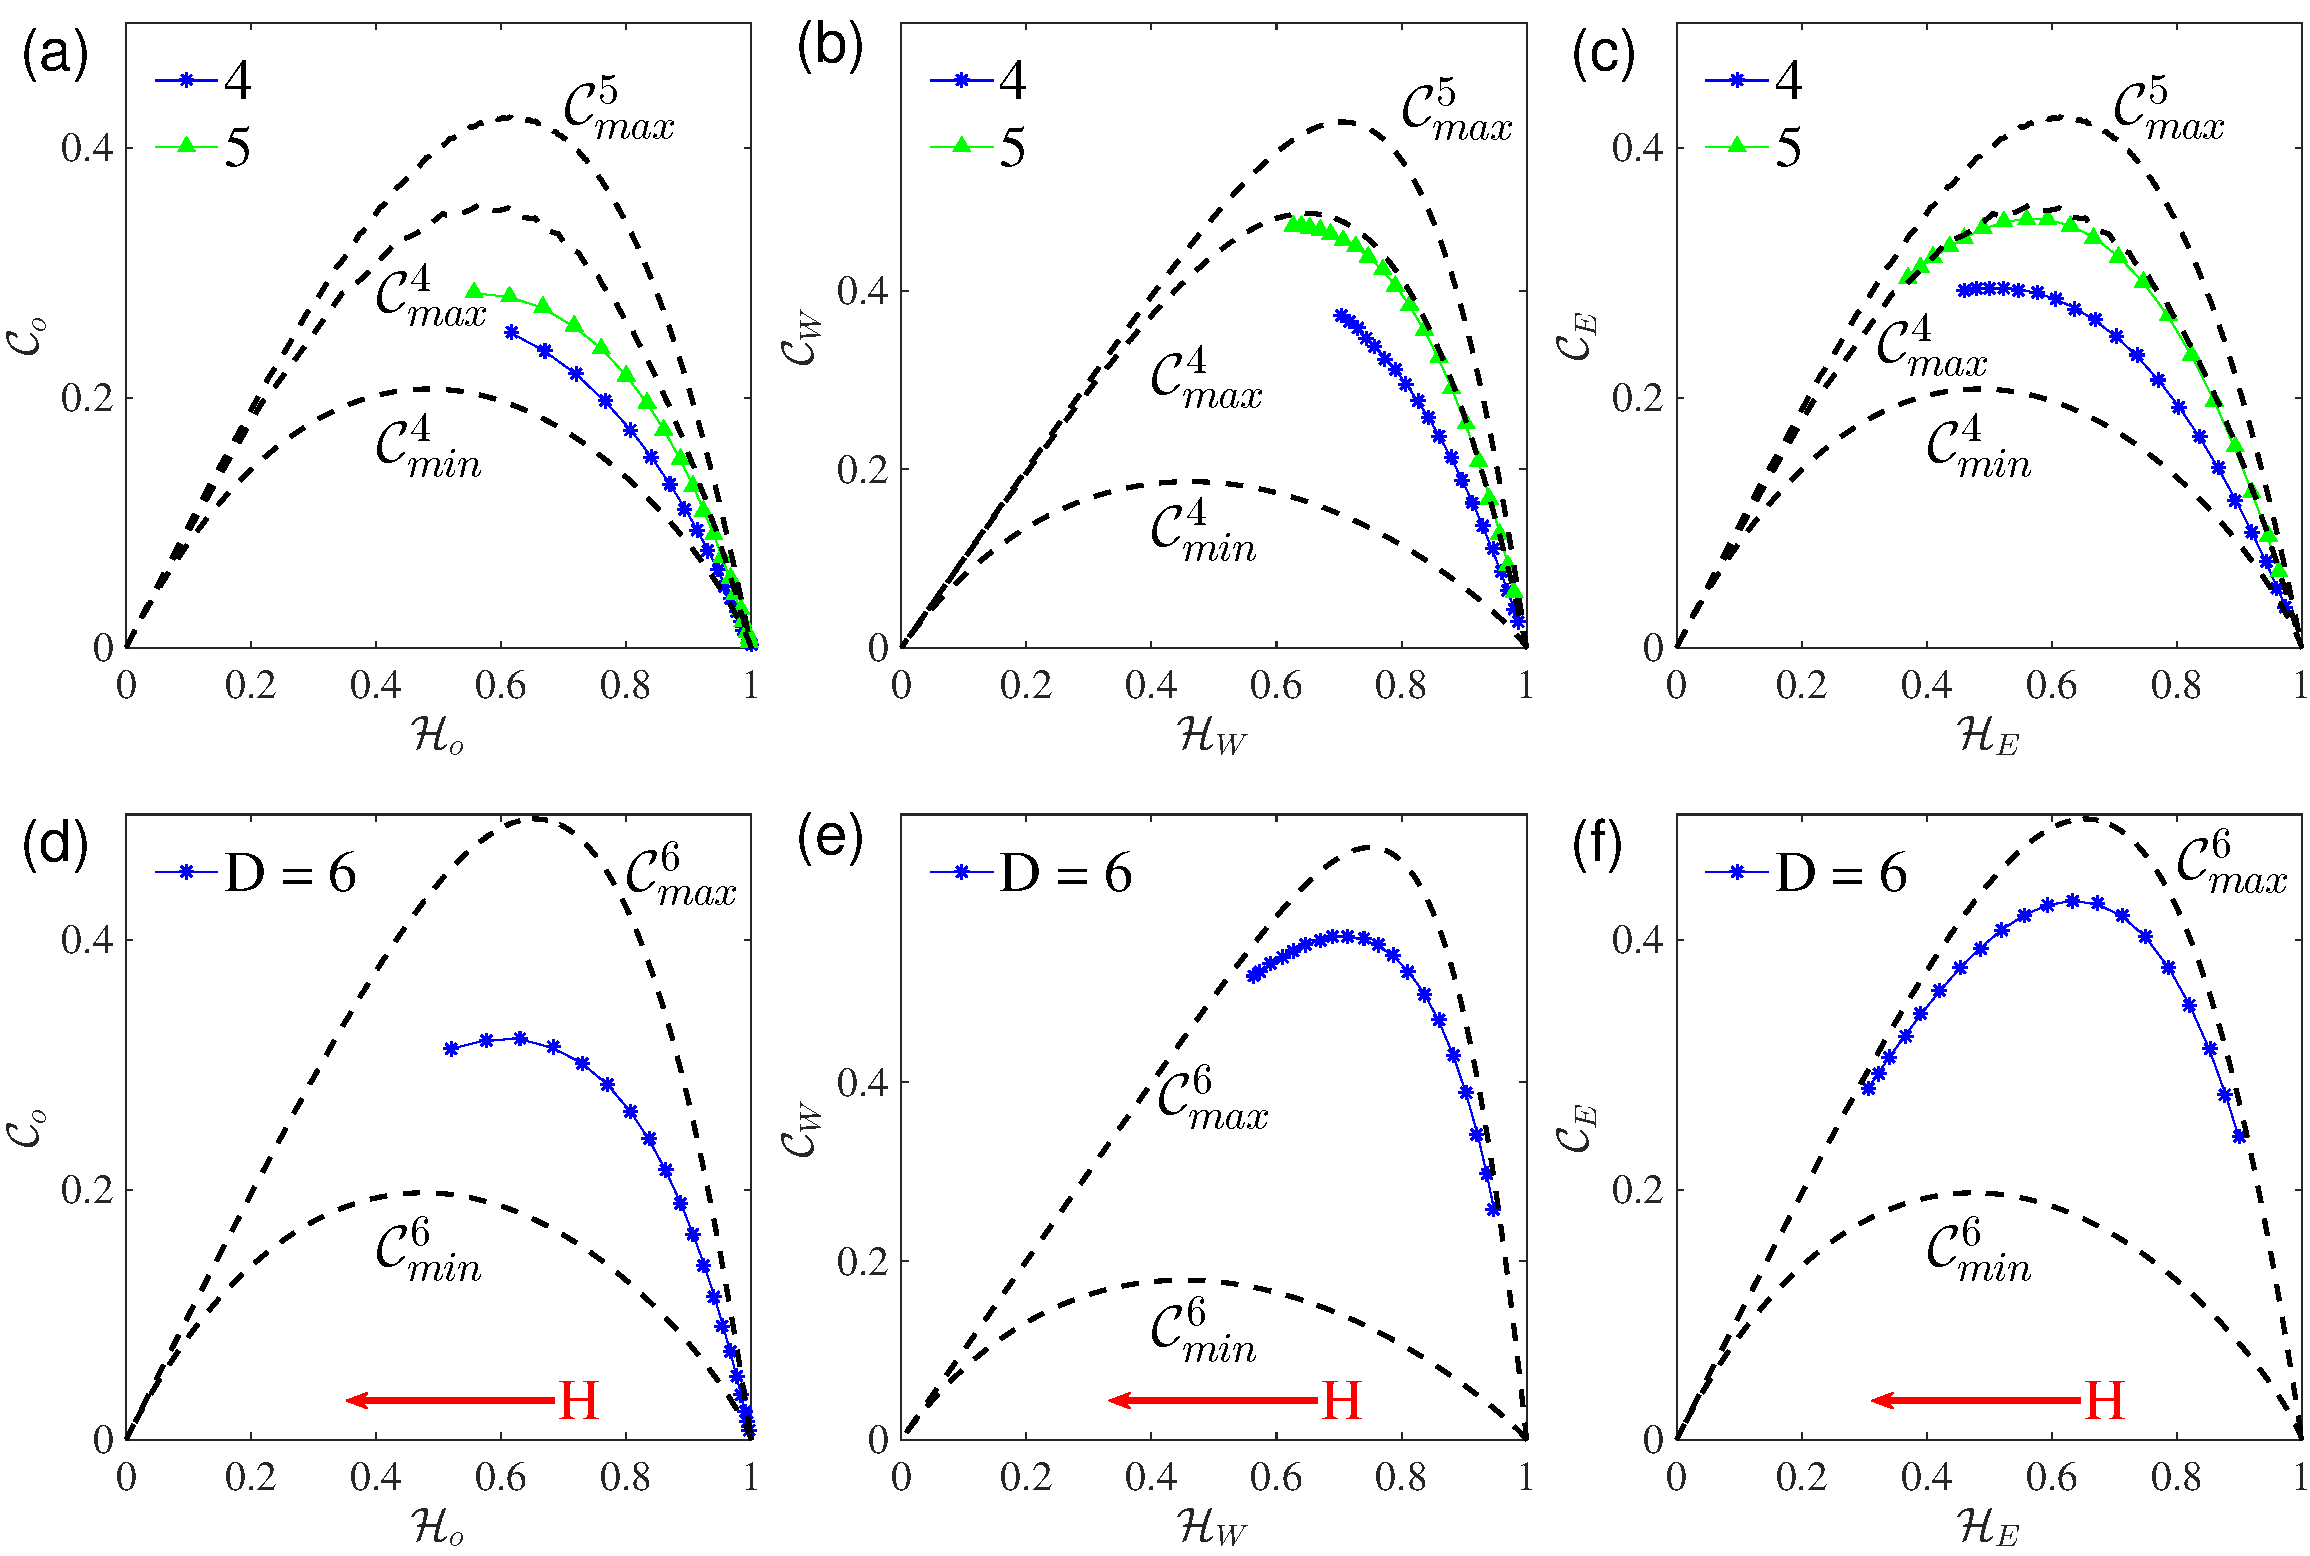
\includegraphics[width=2\columnwidth]{CompEntropy_fBm.pdf}
%\caption{\small{Similar with Fig. \ref{fig:fBmNoise}. Complexity-entropy planes for example series of the fractional Brownian motion for varying Hurst exponent $H$. (a, d) $\mathcal{C}_O$ versus $\mathcal{H}_O$, (b, e) $\mathcal{C}_{W}$ versus $\mathcal{H}_{W}$, and (c, f) $\mathcal{C}_{E}$ versus $\mathcal{H}_{E}$. The dashed lines correspond to the maximum $\mathcal{C}_{max}$ and minimum complexity $\mathcal{C}_{min}$ values for a fixed value of the entropy. (a-c) for embedding $D = 4, 5$ and (d-f) for $D = 6$. }  \label{fig:CompEntrFBM}}
%\end{figure*}

Based on the results of Fig. \ref{fig:fBmNoise}, we conclude that pattern transition behavior provides novel insights for defining SCMs, which complement the traditional SCMs. 

\section{Characterizing dynamical transitions} \label{sec:transi}
The Logistic map experiences various bifurcation scenarios when the control parameter $r$ is systematically increased. However, these dynamical regimes and regime transitions are hidden in the complexity-entropy planes. In this subsection, we aim to expand the figures by showing complexity measures depending on the control parameter $r$. Our motivation is to verify whether SCMs computed from ordinal pattern transition networks are able to detect the dynamical transitions when the control parameter $r$ is varied with a step size $0.001$. Technically, it is a rather simple idea to check whether the normalized entropy $\mathcal{H}$ and SCMs $\mathcal{C}$ are able to track the changes of dynamics. Furthermore, we compare our results with the spectrum of the Lyapunov exponents. 

\begin{figure*}
	\centering 
	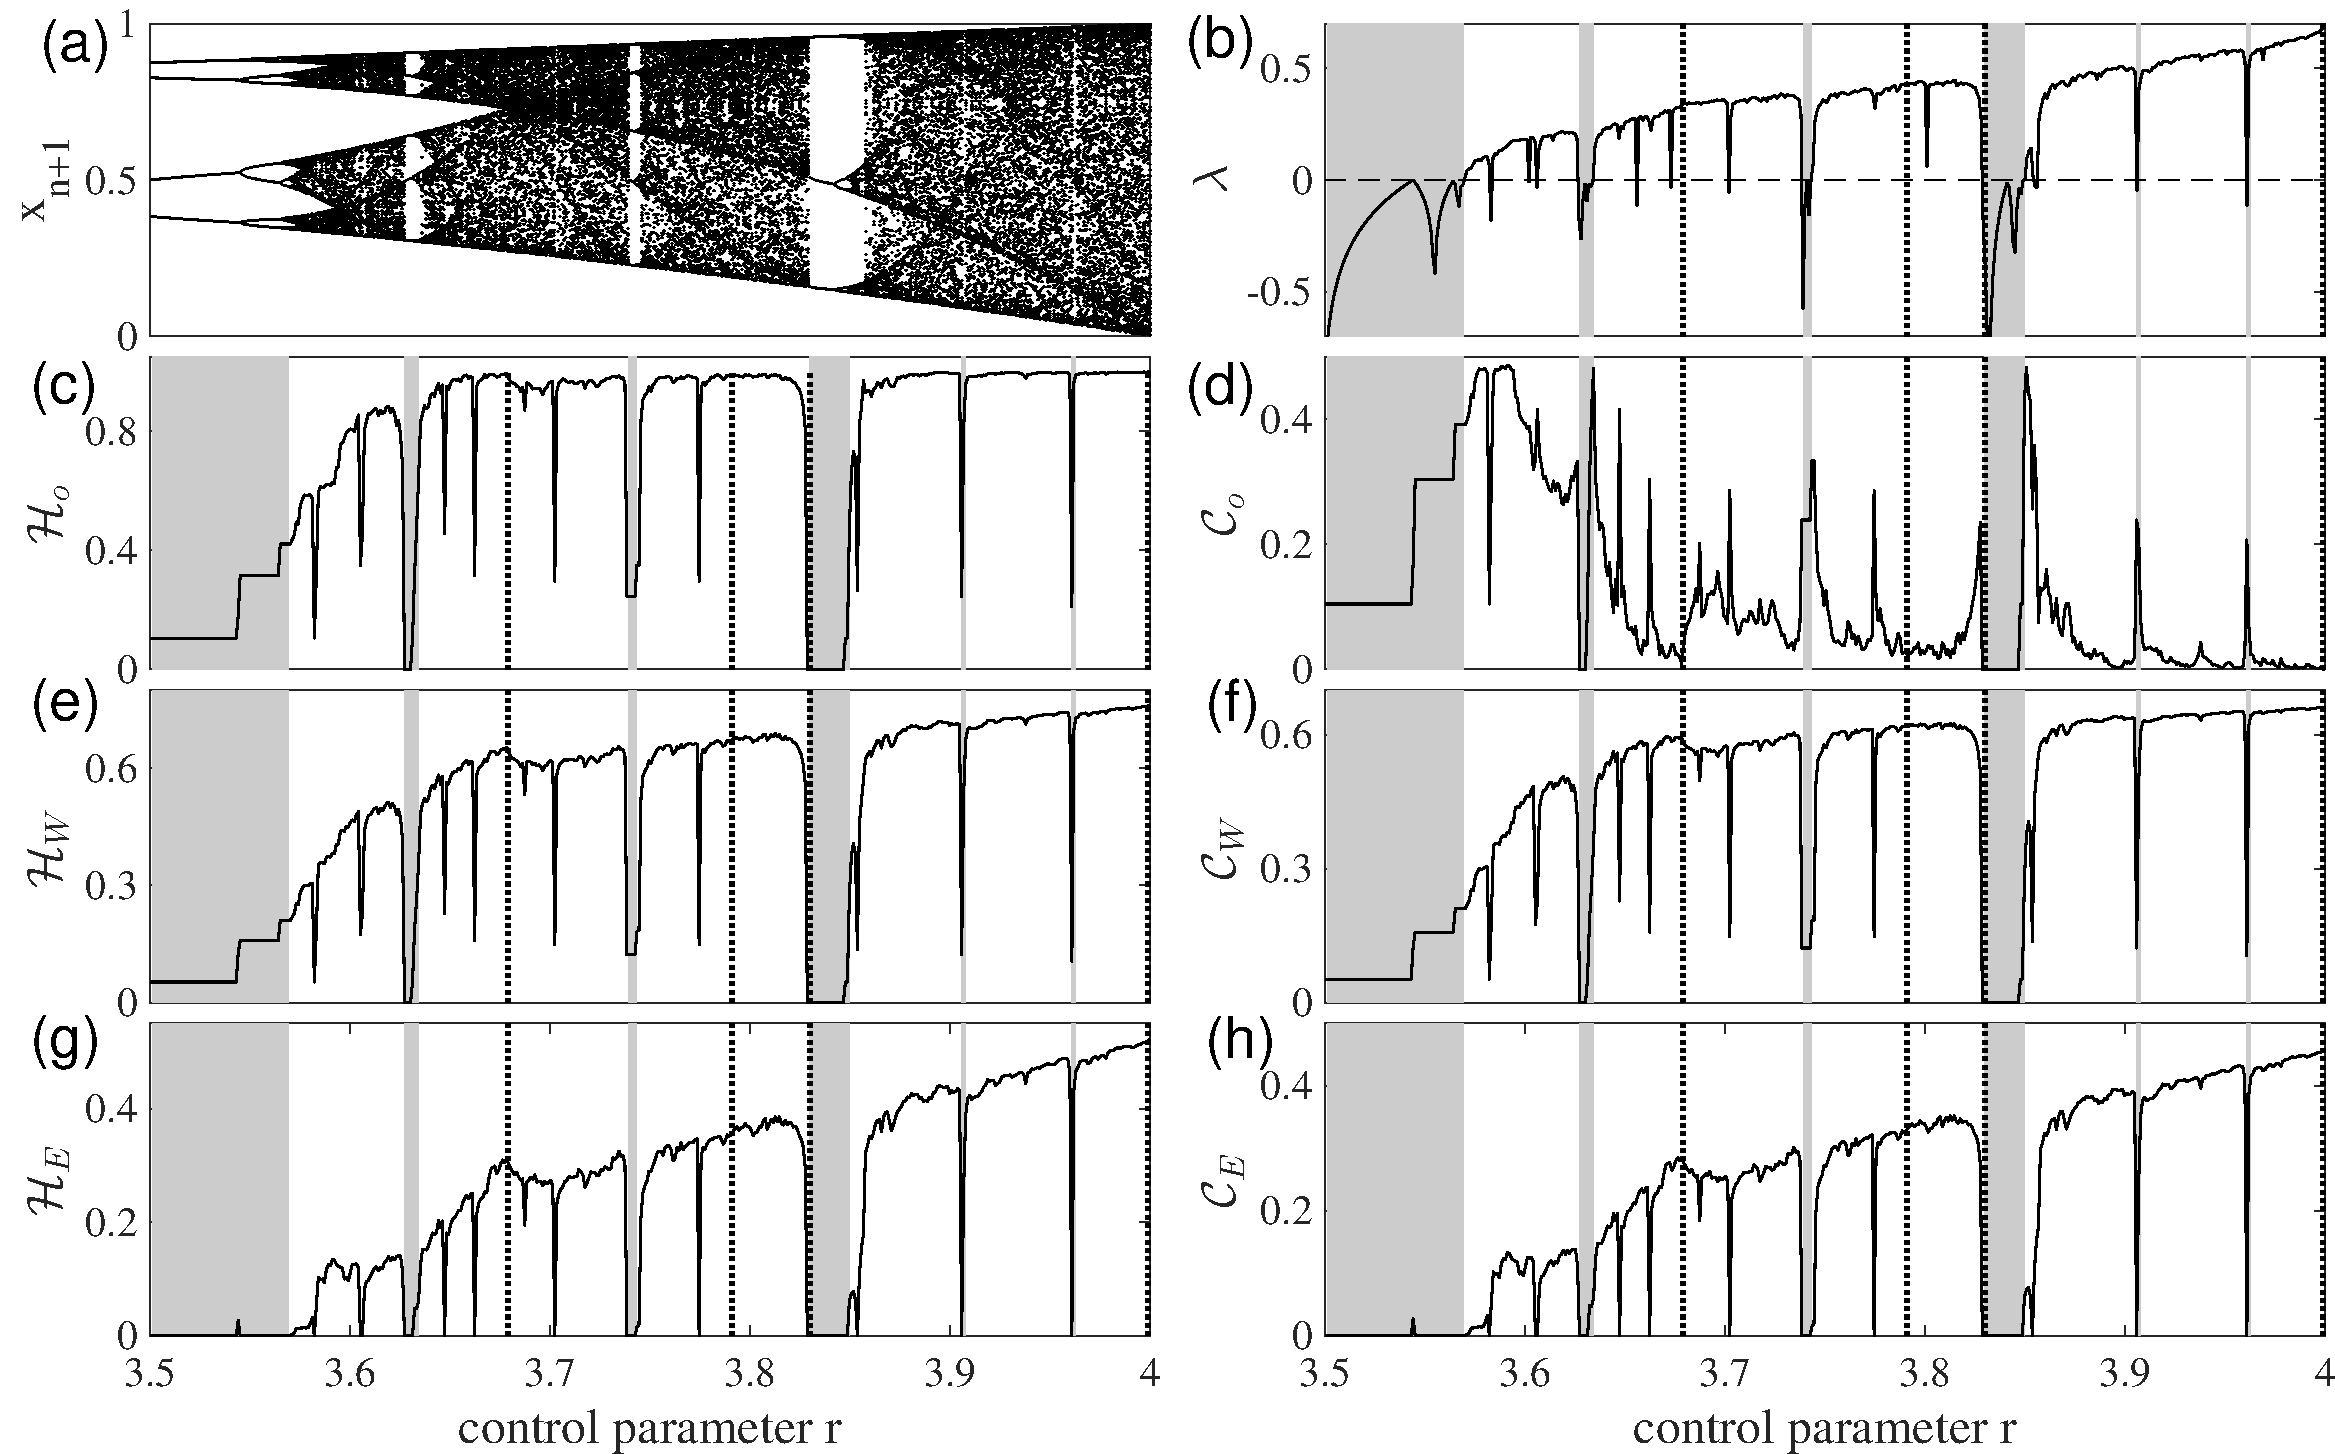
\includegraphics[width=2\columnwidth]{logisticEntropy.pdf}
\caption{\small{Behavior of different statistical complexity measures for the Logistic map in dependence on the control parameter $r$. (a) bifurcation diagram, (b) the spectrum of the maximal Lyapunov exponent, (c) pattern frequency based (permutation) entropy $\mathcal{S}_O$ and (d) complexity $\mathcal{C}_O$; (e) pattern transition frequency based entropy $\mathcal{S}_W$ by the globally normalized weighting matrix $\mathbf{W}$ and (f) the corresponding complexity $\mathcal{C}_W$. (g, h) are entropy $\mathcal{S}_E$ and complexity $\mathcal{C}_E$ which are similar with (e, f) but based on node-wise out-link normalized weighting matrix $\mathbf{W}$. Several major periodic windows have been highlighted by grey background. Vertical dotted lines correspond to the cases summarized in Tab. \ref{tableLog}. } \label{fig:bifurcation}}
\end{figure*}

Overall, all SCMs curves follow the changes in the bifurcation diagram, for instance, showing distinctions in periodic windows  (highlighted by grey color in Fig. \ref{fig:bifurcation}). Except $\mathcal{C}_O$, all other SCMs behave in a much similar manner as the Lyapunov exponents. Namely, as the control parameter $r$ is increased, the chaoticity level grows reaching a maximum at $r = 4$, which, therefore, leads to an increase in the statistical complexity. This similar increasing trend is absent in the case of pattern frequency based complexity measure $\mathcal{C}_O$ (Fig. \ref{fig:bifurcation}(c)). Note that it is a known fact that pattern frequency dependent SCMs often do not follow the growth in the chaoticity in the Logistic map \cite{MartinPLA2003}, which can be improved by Wootter's distance function, instead of the Shannon-Jensen divergence that we used in this work. From this point of view, pattern transition frequency based measures of $\mathcal{C}_W$ and $\mathcal{C}_E$ are more reasonable in the sense that they easily track the growth level of chaoticity. 

There is another improvement for $\mathcal{H}_E$ and $\mathcal{C}_E$ when the Logistic map presents a period doubling bifurcation at $r = 3.544$ (Fig. \ref{fig:bifurcation}(g, h)). The SCMs of $\mathcal{H}_O$,  $\mathcal{C}_O$, $\mathcal{H}_W$ and $\mathcal{C}_W$ show non-zero values in this period doubling window. Furthermore, there are jumps at the bifurcation point $r = 3.544$, which have been also reported in \cite{BandtPRL2002}. To a large extent, the jumps should not be expected because complexity does not change when $r$ passes this point. We show in Fig. \ref{fig:transient} that the iterative transient points are responsible to affect ordinal pattern definitions, which results in the peculiar jumps of SCMs at $r = 3.544$. For estimations from time series of finite length of this work, $\mathcal{H}_E$ and $\mathcal{C}_E$ are not affected seemly. Certainly, we should not over interpret their capabilities since the numerical inaccuracy would be accumulated in a longer iterative process such that different ordinal patterns are identified. In addition, there are many periodic windows of different periods along the axis of control parameter $r$, which prevents us from using a unique predefined number of iterations as initial transients for time series of different period length. 
\begin{figure}
	\centering
	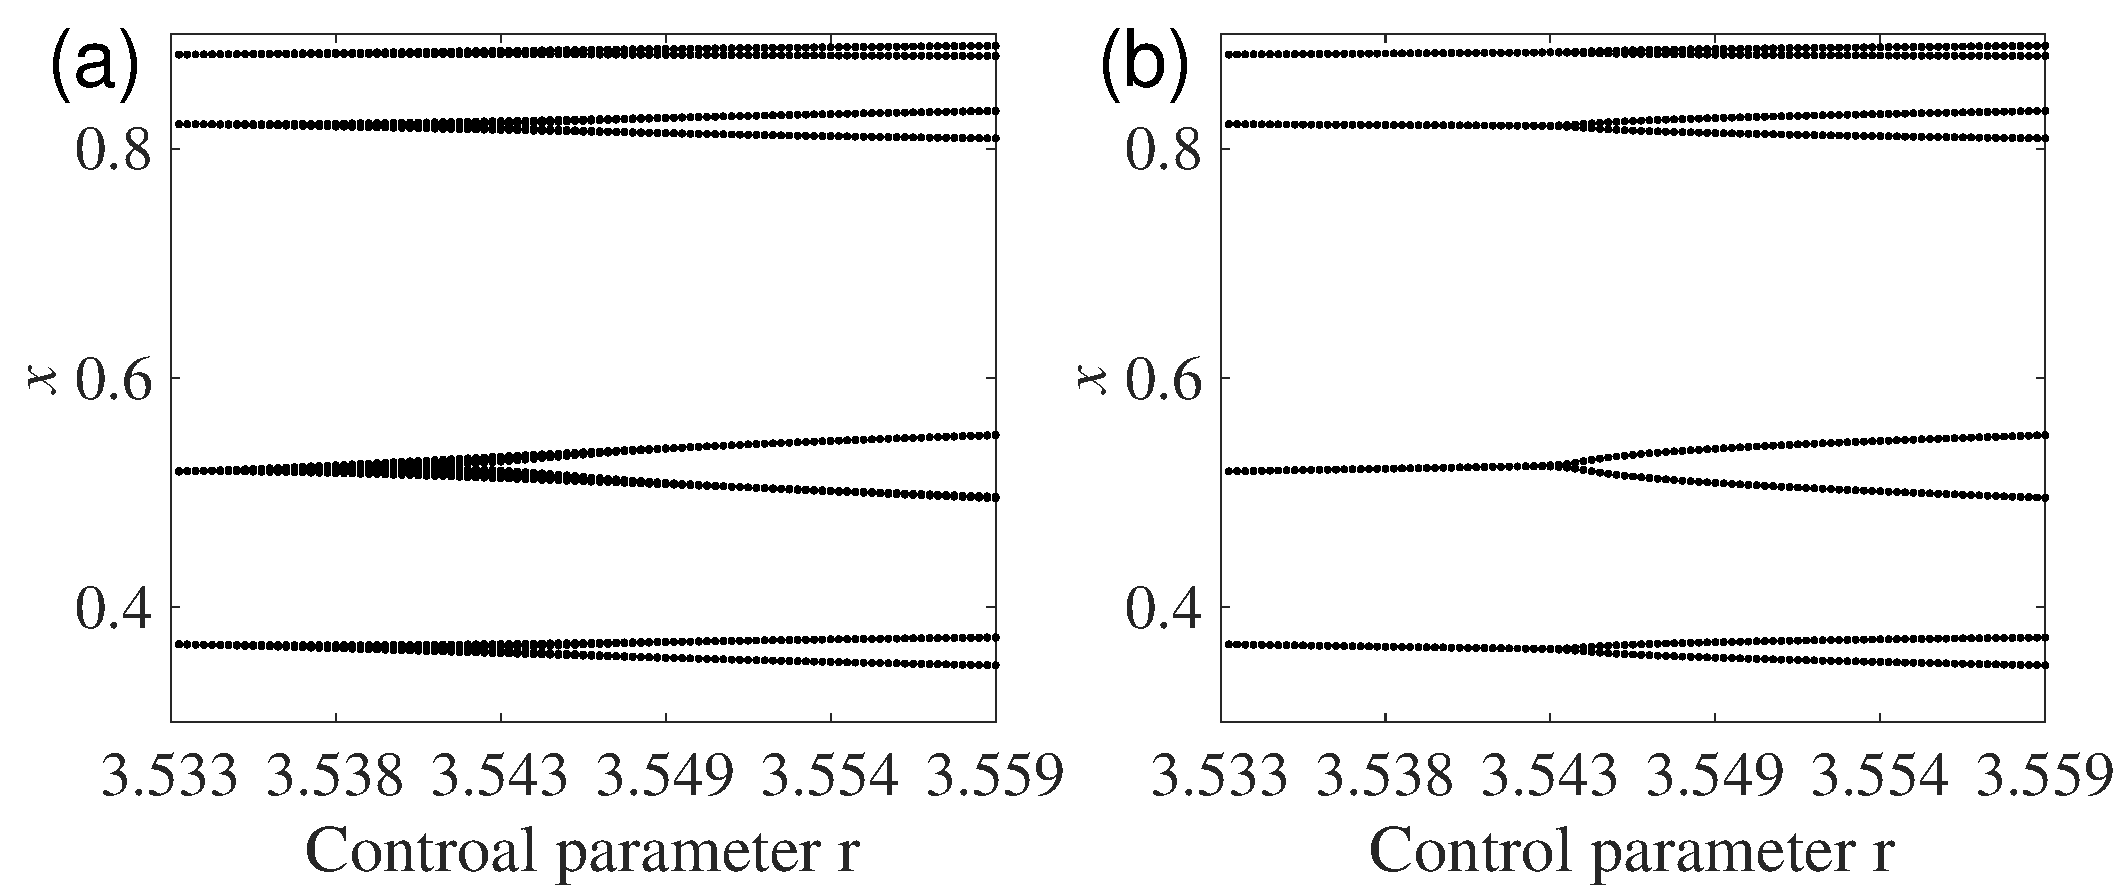
\includegraphics[width=\columnwidth]{period4_exampleTransients.pdf}
\caption{\small{Example to show the transient effects in generating proper bifurcation diagrams of the Logistic map, focusing on the window of period-4 to period-8. The time points get blurred when $r$ is close to $3.544$ when a short transient of $50$ iterates are removed from the analysis (a). In (b) $2000$ initial iterates are removed. }\label{fig:transient}}
\end{figure}
Meanwhile, these jumps have also been observed when the system bifurcates from period-3 to period-6. 

\section{Real time series of fluid flows and ECG} \label{sec:time}
In this section, we use two different experimental time series to demonstrate that SCMs successfully characterize the complexity properties of the underlying systems, showing distinct values for different dynamics. 

The first example is from a laboratory fluid experiment of Baroclinic instability which is used to study patterns of cyclones and anticyclones in climate systems \cite{Read_jfm_1992,ZouEPJST2008}. Depending on the parameters of rotation rate, temperature difference, viscosity and fluid density, this experimental system exhibits a rich variety of flow regimes. In particular, we focus on: (i) {Stable fluid:} the temperature signal of the stable flow exhibits periodic oscillation as the wave drift patterns arrive at the measured fixed point. (ii) {Quasi-periodic 2- frequency Amplitude vacillation (AV-2):} this case is identified as a 2-frequency quasi-periodic amplitude flux. The wave drift is composed of slow and regular oscillations in the temperature signal, but a fast modulation in the amplitude is also visible. AV-2 is characterized by periodic growth and a drop in wave amplitude with little change in waveform. (iii) {Quasi-periodic 3-frequency amplitude vacillation (AV-3): } We also analyze a quasi-periodic 3-frequency amplitude vacillation (AV-3) time series which is obtained from a three-dimensional direct numerical simulation in an air-filled rotating Baroclinic instability experimental \cite{Read_jfm_1992}. (iv) {Modulated amplitude vacillation (MAV):} this case is identified as a low-dimension stream, chaotically modulated and with waves of varying amplitudes. Amplitude modulation results in a complex temperature signal.

The second example time series comes from the physiological signals of human electrocardiogram (ECG) recordings that are collected from patients in a Coronary Care Unit and the Creighton University Cardiac Center. Ventricular arrhythmia are a very significant but poorly understood dynamical system, showing rich nonlinear properties. In this work, we focus on three different states: normal sinus rhythm (SR), ventricular tachycardia (VT) and ventricular fibrillation (VF) \cite{smallCSF2002}. From the data bank of recordings of ECG during various rhythms, we selected 14 time series showing sinus rhythm (SR) prior to onset of arrhythmia, 12 time series of VT and 17 VF. The ECG recordings have been annotated with SR, VT and VF by skilled cardiologists on the basis of waveform morphology. Each recording consists of at least $10,000$ data points (20s) in length and 250 Hz in sampling frequency. 

For choosing embedding parameters for both example time series, we follow the suggestions that are proposed in the respective literature \cite{ZouEPJST2008,smallCSF2002}. Although we are facing with the inevitable presence of non-stationary and noise in the experimental data, we have verified that the following results do not change significantly while embedding parameters are varied. In particular, we have treated embedding dimension as a free parameter which is varied in the interval as $D = 2, 3, \dots, 7$, while the embedding delay $\tau$ is the following. In the case of temperature time series from the fluid flows, embedding delay $\tau_{i} = 218s$ for stable solution, $\tau_{ii} = 136.5s$  for AV-2, $\tau_{iii} = 185.625$s for AV-3, and $\tau_{iv} = 118s$ for MAV. In the case of recordings of ECG time series, embedding delay $\tau = 5$. The results have been averaged over all subjects. 

Generally speaking, the OPTN based statistical complexity measures of both the flow data and the ECG recordings enhance our understanding of the underlying nonlinear system, which are shown in Fig. \ref{fig:fluid}. More specifically, in the case of fluid data (Fig. \ref{fig:fluid}(a)), complexity measures of $\mathcal{H}_O$, $\mathcal{H}_W$, $\mathcal{C}_W$, $\mathcal{H}_E$ and $\mathcal{C}_E$ show consistent complexity values for stable wave solution (SW), quasi-periodic 2-frequency Amplitude vacillation (AV-2), quasi-periodic 3-frequency Amplitude vacillation (AV-3) and chaotic modulated amplitude vacillation (MAV). Namely, the complexity of these four cases has the following order: SW has the smallest complexity since it shows periodic oscillation of trivial recurrences, while MAV has the highest complexity since it is chaotically modulated amplitude vacillation. Quasiperiodic states show inter-mediate complexity values since these two cases have non-trivial recurrences but with low complexity. Interestingly, AV-3 presents higher complexity than AV-2. The relationship of complexity between periodic, quasiperiodic and chaotic solutions still holds for $\mathcal{C}_O$ although the corresponding values become comparable. In particular, it becomes hard for $\mathcal{C}_O$ to tell the difference between AV-2 and AV-3. 

Qualitative similar results have been obtained for ECG recording series (Fig. \ref{fig:fluid}(b)). Clearly, different ECG recordings exhibit remarkably distinct complexity values. Specifically, SR recordings show pronounced highest complexity values of $\mathcal{H}_O$, $\mathcal{H}_W$, $\mathcal{C}_W$, $\mathcal{H}_E$ and $\mathcal{C}_E$ since there are rather broad frequency bands between 50 and 100 beats/min in the signals \cite{smallCSF2002}. On the other hand, the complexity of VT has the smallest values comparable to the case of VF. Similarly to the case of flow data, SR shows the smallest value of $\mathcal{C}_O$ while VT and VF have comparable values that are relative higher than SR. 
\begin{figure*}
	\centering 
	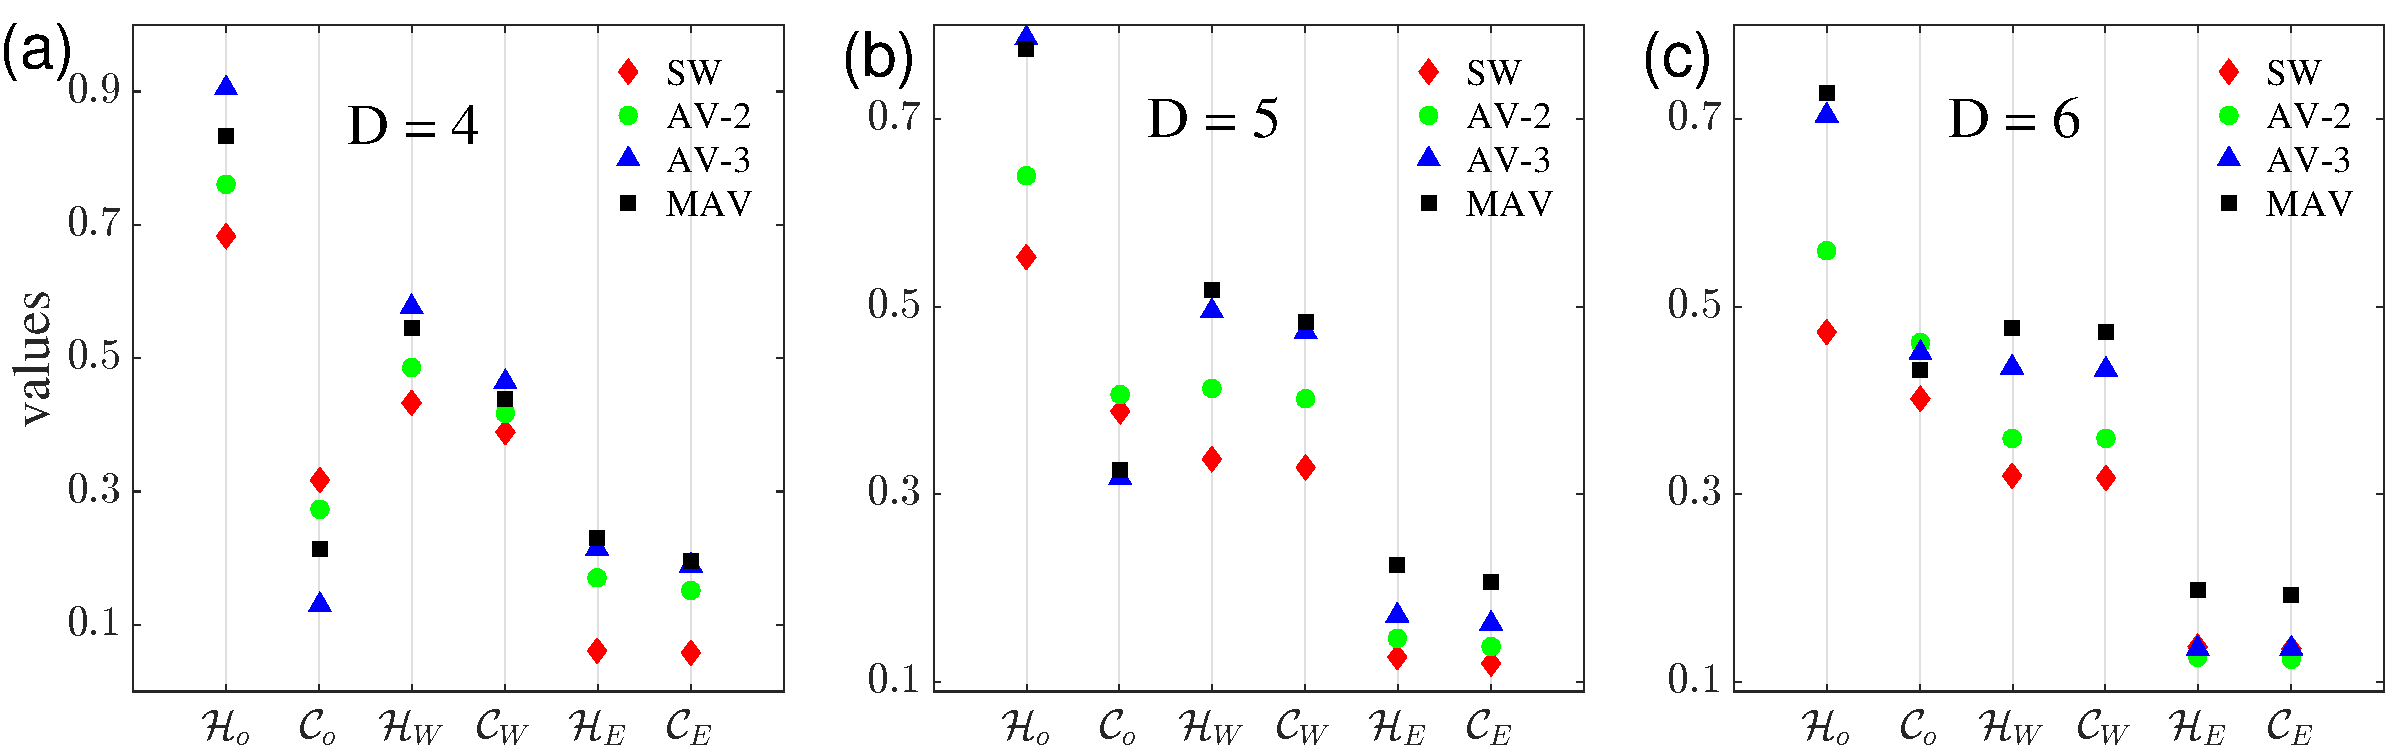
\includegraphics[width=2\columnwidth]{fluidExample.pdf}
\caption{\small{Application of SCMs to experimental fluid data (a) and human recordings of ECG (b). The results have been averaged over embedding delays $D = 2, 3, \dots, 7$. In (a), stable wave (SW) $\blacklozenge$, quasiperiodic 2-frequency amplitude vacillation (AV-2) $\bullet$, quasiperiodic 3-frequency amplitude vacillation (AV-3) $\blacktriangle$, and chaotic modulated amplitude vacillation (MAV) $\blacksquare$. In (b), normal sinus rhythm (SR) $\blacktriangle$, ventricular tachycardia (VT) $\blacklozenge$ and ventricular fibrillation (VF) $\bullet$. } \label{fig:fluid}}
\end{figure*}


\section{Discussions} \label{sec:con}
complex network approaches for nonlinear time series analysis \cite{ZouPR2018}. 

Some open problems regarding to the ordinal pattern analysis need to be further explored. Length dependence, further numerical performance to show distinctions between different dynamics (various models of maps, long range correlated fractional Brownian motion, fractional Gaussian noise etc)

For periodic windows of the Logistic map, one may use longer data lengths, but does not improve the estimate very much. 

Generalization from univariate to bivariate time series analysis will be further discussed. We noticed that this remains to be a largely untouched area for statistical complexity analysis. It would be an interesting task to show the dependence of complexity on interaction. 

\section{Acknowledgements}
Parts of this work have been financially supported by the National Natural Science Foundation of China (Grant No. 11872182 and 11835003). Y. Z. further acknowledges the support by Shanghai Municipal Science and Technology Major Project (No.2018SHZDZX01) and ZJ Lab. 

\bibliographystyle{unsrt}
\bibliography{ref_Zou}

\end{document}
